\section{Ridge Regression}
\subsection{Implementation and experiments}
We implemented a function {\tt ridgeRegression} that, given a maximum degree $M$ and a regularization parameter $\lambda$ computes the polynomial ridge regression. Mathematically, we want to minimize in $w$ the following expression:
\begin{equation*}
    \|A\mathbf{w} - \mathbf{y}\|^2 + \lambda \|\mathbf{w}\|^2
\end{equation*}
Where $w$ are the polynomial coefficients, $x$ the vector of data points and $A$ a matrix such that:
\begin{equation*}
    A_{i,j} = x_i^{j-1}, \qquad \forall \, 1 \leq i \leq n, \, 1 \leq j \leq M+1
\end{equation*}
We experimented the ridge regression on the simple data from Bishop's Figure 1.4. Figure~\ref{fig:ridge1} presents a few examples. the two top figures show that with $\lambda = 0$ we indeed have the usual least-square regressions. In particular we notice the overfitting when $M=10$. Now, for the two bottom figures, we keep $M =10$, and we show how different values of parameter $\lambda$ can control the overfitting of the solutions. The higher $\lambda$ is, the smaller the polynomial coefficients are, and as a consequence the more we avoid the overfitting. But we would need a validation dataset in order to find an optimal value for $\lambda$. Here $\lambda = 0.005$ seems to be correct, and $\lambda = 1$ leads to under-fitting.

\begin{figure}[h]
  \centering
 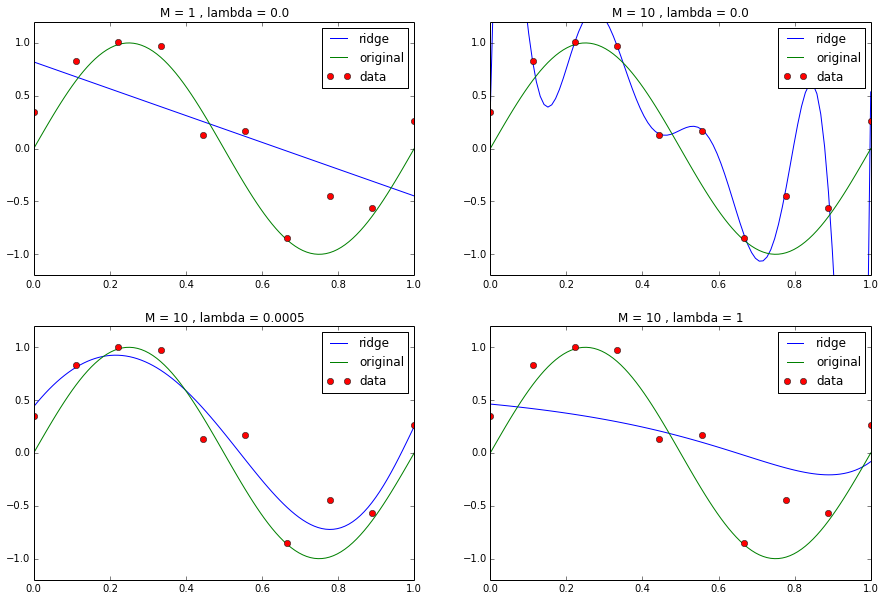
\includegraphics[width=10.3cm]{../Figures/Q3/ridge1.png}
\caption{Ridge regression for various $M$ and $\lambda$. The green curve represents the original $\sin$ function used to generate the red datapoints}
\label{fig:ridge1}
\end{figure}

\subsection{New dataset and grid-search}
We use the same method with the new dataset. But this time, we are given a validation set. We use it to optimize the value of the parameters $M$ and $\lambda$, using the grid-search technique:
\begin{enumerate}
    \item We create a grid of the parameters we want to test: for example $M \in [2,4,6,8]$ and $\lambda \in [10^{-2},10^{-1},1,10]$
    \item Perform the ridge regression with all these parameters.
    \item Compute the $SSE$ (here divided by the number of sample) on the validation set.
    \item Go back to step 1 with a finer grid around the optimal value.
\end{enumerate}
Figure~\ref{fig:ridge2} shows four different sets of parameters and the corresponding regressions and validation errors. The first one is the most simple case of pure affine least-square regression, good to compare the validation error.  The second and third graphs represent the effect of the parameter $\lambda$ on the solution. We can see that with the small $\lambda$, overfitting leads to a terrible validation error. The result of the grid-search for best parameters is plotted in the last figure, with $M=4$ and $\lambda = 0.83$.

We notice that ridge does not seem good at handling outliers. Indeed, in this example, we can see that the square error forces the curve fitted to the training set not to be too far from the outlier. Furthermore, this is also an interesting example of overfitting on the validation set. Indeed, the last curve performs extremely well on the validation set (green points), but fails to do so on the testing set, with an mean square error of $2.76$. One solution would be to remove the outliers before performing regression. Next section will also provide another solution.

\begin{figure}[h]
  \centering
 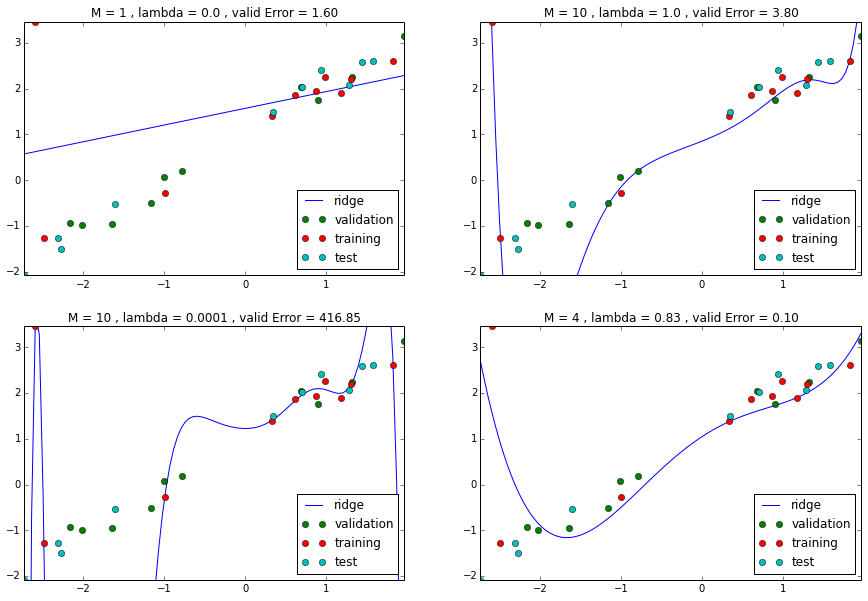
\includegraphics[width=10.3cm]{../Figures/Q3/ridge2.png}
\caption{Ridge regression for various $M$ and $\lambda$. The fit is done on the training set (with one outlier) and the error is computed on the validation set.}
\label{fig:ridge2}
\end{figure}

\subsection{Application on BlogFeedback data}
We use the exact same method of grid-search as in the last question. It is now easier to plot. In Figure~\ref{fig:grid} we plot the averaged square error on the validation set, depending on the value of $\lambda$. It is now easy to see how we evaluated $\lambda = 10^{2.95}$ to be the best choice.
\begin{figure}[h]
  \centering
 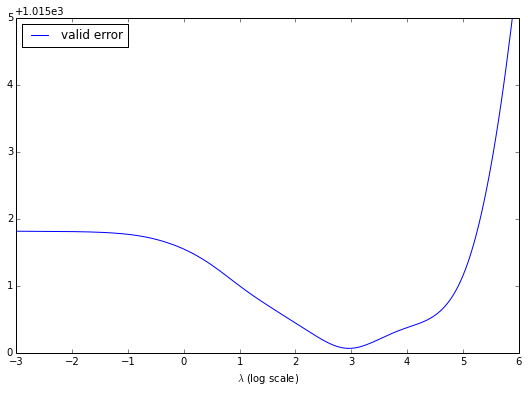
\includegraphics[width=8cm]{../Figures/Q3/grid.png}
\caption{Grid-search for parameter $\lambda$. The y-axis is the mean-squared validation error and the x-axis is $\log_{10}(\lambda)$ .}
\label{fig:grid}
\end{figure}

Here is a summary our mean-square error results using this parameter with our linear model:
\begin{center}
  \begin{tabular}{| c  | c |c |}
    \hline
 Learning set MSE & Validation set MSE &  Test set MSE \\ \hline
 884.97  &  1015.07 & 896.37 \\
    \hline
  \end{tabular}
\end{center}
The fact that the test set MSE is almost as low as the one on the training set is a good sign that we managed to avoid overfitting.

We have applied two scaling processes on the features, as seen in the wikipedia article:
\begin{itemize}
    \item Resampling : $x' = \frac{x - \min(x)}{\max(x)-\min(x)}$
    \item Standardization: $x' = \frac{x - \mu}{\sigma}$
\end{itemize}
\begin{center}
  \begin{tabular}{| c | c  | c | c |}
    \hline
 Scaling &  Learning MSE & Validation MSE &  Test MSE  \\ \hline
 Resampling & 881.63  &  1015.23 & 894.52 \\
 Standardization & 927.78  &  1062.48 & 941.85 \\
    \hline
  \end{tabular}
\end{center}
Though standardization does not seem to help, we have slightly better results after resampling. (note that we have proceed to a grid-search to find the best value for $\lambda$ for each scaling method).
